\section{Paid Incentives in Signals}
\subsection{Motivation}
DAOs often face low participation: most holders do not see sufficient upside to engage, and reputational risk pushes signaling to the last minute. Some DAOs spend \$1M+ per year on delegate programs. Signals inherits similar participation risks, so we add configurable incentives that reward early, accurate support and penalize weak or misaligned signaling.

\subsection{Mechanism 1: General Participation Incentives (IncentivesPool)}
A shared \texttt{IncentivesPool} can fund supporters of any initiative that gets accepted. The pool is independent from boards and can be shared across many (1:M). Its reward token is immutable and specified in the constructor; funds are added with \texttt{addFundsToPool}. Boards must be explicitly approved with two parameters: a per-board \emph{max budget} and a \emph{totalRewardPerInitiative} cap. Boards then link to the pool \emph{before} they open.

When supporters add locks, the board records each lock's \emph{incentive credit} in the pool using the lock's time-weighted contribution at creation. Credits are aggregated into a fixed number of time buckets (default: 24) with a starting interval (default: 1 hour). The board provides an \emph{incentive curve} configuration (linear today, 2--24 parameters), and the pool converts the curve into per-bucket multipliers via interpolation and normalization. On redemption after acceptance, the board requests the pool to pay rewards for the redeeming locks: each lock gets a share proportional to its credited bucket and the curve's multipliers. The pool enforces the per-initiative cap and the board's remaining budget; if depleted, payouts simply become zero without blocking acceptance or redemption.

\begin{itemize}[leftmargin=*]
  \item \textbf{Setup}: deploy pool with \texttt{REWARD\_TOKEN}, fund with \texttt{addFundsToPool}, approve boards with \texttt{approveBoard(board, boardBudget, totalRewardPerInitiative)}, link from the board before opening via \texttt{setIncentivesPool}.
  \item \textbf{Accounting}: time is bucketed and compressed (if buckets fill, they are reduced in-place to keep a bounded history).
  \item \textbf{Safety}: only approved boards can record credits and claim. Claims respect budgets and never revert for insufficient pool balance; rewards may be 0 if exhausted.
\end{itemize}

\subsection{Mechanism 2: Sponsored Initiative Incentives (Bounties)}
Anyone can add rewards to a specific initiative via the \texttt{Bounties} contract. Tokens must be on a \texttt{TokenRegistry} maintained by role-based access control. Bounties are stored with amount, optional expiration, and distribution \emph{splits} configured by the owner (e.g., protocol/treasury/supporters). On acceptance, bounties are aggregated by token and split according to the active version of the configuration, crediting internal balances for recipients. Current limitations: refunding expired bounties is a planned enhancement and is not fully implemented yet.

\subsection{Impact}
Rewards amplify Signals’ core design: only positive support, opportunity cost via locks, and time-weighted influence that lets smaller holders compete. Incentives raise the cost of frivolous signaling and make early, accurate support economically meaningful, improving resilience against brigading or apathy-driven noise.

\begin{figure}[h]
  \centering
  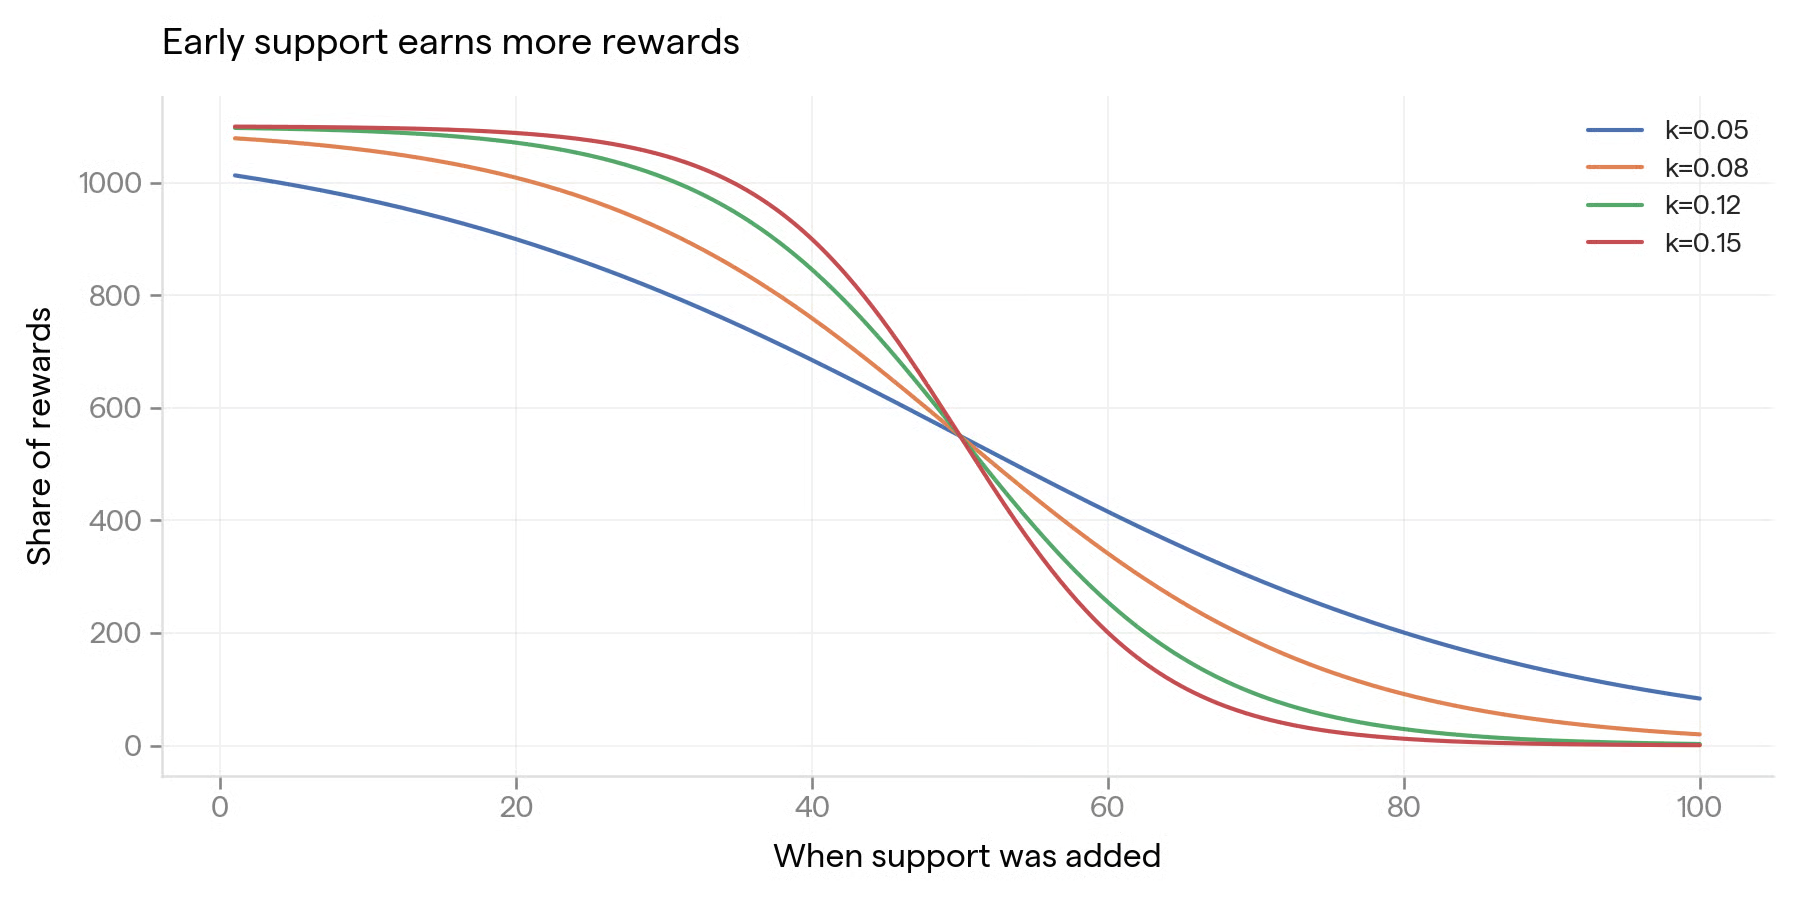
\includegraphics[width=0.85\linewidth]{figures/fig-rewards.png}
  \caption{Example reward distribution emphasizing early supporters via bucket multipliers and shared upside.}
\end{figure}

\subsection{Implementation Notes (from Tests)}
End-to-end tests validate:
\begin{itemize}[leftmargin=*]
  \item Linking a board to a pool must happen before the board opens; otherwise calls revert.
  \item Reward distribution with a single supporter pays the \texttt{totalRewardPerInitiative} cap (subject to remaining budget).
  \item With multiple supporters at different times, earlier buckets receive higher multipliers (per linear config) and split rewards accordingly.
  \item Pool depletion is non-blocking: acceptance and redemption succeed; claims pay zero if budgets are exhausted.
\end{itemize}
